%!TEX TS-program = xelatex
% Much of the initial version of this lab manual was taken from Jonathan Peelle's lab manual. 
% See original source here: https://github.com/jpeelle/peellelab_manual/

\documentclass[letterpaper,11pt,oneside]{memoir}
\usepackage{color}

%\setromanfont{Cambria}
\usepackage{xunicode,fontspec,xltxtra} 
\usepackage{libertine} 

\usepackage[pdftitle={Smith Lab Manual}, pdfauthor={David V. Smith}, colorlinks=true, urlcolor=blue]{hyperref}

\usepackage{multicol}
\usepackage{array,ragged2e}
\usepackage{fontspec,xunicode}
\defaultfontfeatures{Mapping=tex-text}



\definecolor{shadecolor}{gray}{0.9}
\setsecnumdepth{section}
\maxtocdepth{subsection}
\usepackage{multicol}
\usepackage{enumitem}

\usepackage{xurl}
\usepackage{csquotes}


\renewcommand{\UrlFont}{\ttfamily\footnotesize}

\chapterstyle{article}



%\pretitle{\huge\sffamily}
%\posttitle{\vskip 0.5em}
% \preauthor{\begin{flushleft}}
%\postauthor{\end{flushleft}}
%\predate{\begin{flushleft}}
 %\postdate{\end{flushleft}}

\setlength{\droptitle}{1in}

\checkandfixthelayout	% for memoir class

\begin{document}


\title{Smith Lab Manual\thanks{Code and version history: \url{https://github.com/DVSneuro/smithlab_manual}}}
\author{David V. Smith\\Department of Psychology and Neuroscience\\Temple University}
\date{\today}

%\href{https://sites.google.com/a/temple.edu/dvs-lab/SmithLab\_manual.pdf}{Link to Lab Manual}

\maketitle

\pagestyle{titlingpage}


\cleardoublepage
\frontmatter
\tableofcontents
\cleardoublepage

\mainmatter

\pagestyle{headings}

%%%%%%%%%%%%%%%%%%%%%
\chapter{Introduction}
My overarching goal is to foster an environment of scientific excellence and personal development for the lab. We should all continually strive to learn and improve. And we should try to have fun doing great science that makes a difference in our fields and our broader communities. This lab manual\footnote{Parts of this document are derived from Dr. Jonathan Peelle's excellent \href{https://github.com/jpeelle/peellelab\_manual/}{Lab Manual}.} is meant to be the first resource for the lab as we seek to achieve these goals. You can also find the lab here:

\begin{itemize}[noitemsep]
\item Website: \url{https://sites.temple.edu/neuroeconlab/}
\item GitHub: \url{https://github.com/DVS-Lab}
\item Twitter: \url{https://twitter.com/DVSneuro}
\item OSF: \url{https://osf.io/5zq6h/}
\end{itemize}

\noindent There are also a couple of sites accessible only by lab members:

\begin{itemize}[noitemsep]
\item Asana: \url{https://app.asana.com}
\item Slack: \url{https://smithlab-workspace.slack.com}
\item Slab: \url{https://smithlab.slab.com/}
\end{itemize}

In general, firm policies are in the lab manual, whereas ways of implementing those policies (i.e., getting stuff done) should be on Slab (a.k.a., the wiki) so that they can be updated by anyone in the lab. Asana organizes tasks that need to be completed and relevant notes/discussions. And Slack facilitates group communication, announcements, and quick, informal chats. Any information that is potentially private or sensitive should go in a protected location. (You can read more about various lab resources in \Sref{sec:communicationInLab} on \pref{sec:communicationInLab}.)

\begin{shaded}
\noindent I assume that this lab manual and any documentation on Slab are accurate and clear. This means that you should follow all of the policies and protocols in this manual and Slab. If you notice something that seems to be wrong (or missing), please let me know (for the lab manual) or change it yourself (for the wiki). If there is something in the lab manual or wiki that you notice people aren't doing, please bring this up at lab meeting, or to me, privately---don't assume this is okay (it's not). 
\end{shaded}

Note, although I don't think there are any cases where my lab policies conflict with Temple policies (please do let me know if you find otherwise), let's be clear that Temple policies supersede lab policies in all cases and you are responsible for knowing those policies. For instance, I defer to Temple on matters relating to COVID exposures and ADA-related accommodations, among many other things.


%%%%%%%%%%%%%%%%%%%%%
\chapter{About the Lab} 
You should think of the lab as a small business, complete with operating costs and the demands to allocate resources (i.e., time and funding) efficiently in order to maximize returns. Our principal products include a) rigorous scientific publications that describe what we've learned about the world (and our materials and data) and b) highly-skilled trainees. Of course, these products are deeply intertwined in the sense that publications don't happen without skilled trainees and some skills are difficult to showcase without a corresponding publication.

\section{Our Values}

\subsection{Respect for Diversity}
As a first-generation college student from a low-income area of South Carolina, I am fortunate to be running a lab at an R1 university. It is my intent that trainees from diverse backgrounds and perspectives be well served by this lab, that trainees’ learning needs be addressed both in and out of the lab, and that the diversity that trainees bring to this lab be viewed as a resource, strength and benefit. It is my intent to present materials and activities that are respectful of diversity: gender, sexuality, disability, age, socioeconomic status, ethnicity, race, and culture. Your suggestions are encouraged and appreciated. Please let me know ways to improve the effectiveness of the lab for you personally or for other trainees. In addition, if any of our meetings conflict with your religious events, please let me know so that we can make arrangements for you.

\subsection{Impactful Science}
We're all here to do great science (and hopefully have fun in the process). We want our work to make an impact in our field and our broader community. We want others to be able to learn and improve based on the work that we do. As you're working on your projects, think about how your work could be used by other scientists. And, think about how the broader community will receive your work. 

\subsection{Skillset Development}
It is my hope that everyone will aim to continually develop a full spectrum of skills, from hard skills (e.g., technical and analytical) to soft skills (e.g., communication and teamwork). Notably, this goal has been discussed at NIH\footnote{\url{https://loop.nigms.nih.gov/2015/11/catalyzing-the-modernization-of-graduate-education/}} and has been argued to promote transferable skills\footnote{\url{https://science-latte.com/infographics/\#jp-carousel-4019}}. Consider the following areas and examples: 

\begin{figure}
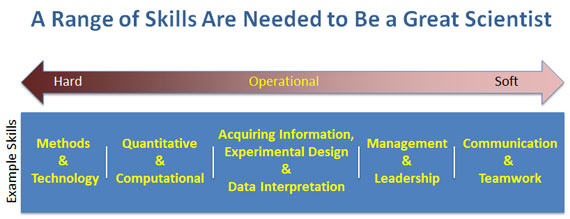
\includegraphics[width=\textwidth]{figures/skillrange.jpg}
\caption{A full spectrum of skills are needed to become a great scientist in academia or industry. Figure taken from the National Institutes of Health (NIH; see \href{https://loop.nigms.nih.gov/2015/11/catalyzing-the-modernization-of-graduate-education/}{link} for more information).}
\end{figure}


\begin{itemize}[noitemsep]
\item \textbf{Methods \& Technology}: You have a deep understanding of how your tools work. And, you appreciate their strengths and weaknesses for addressing specific questions and issues in your areas of interest.
\item \textbf{Quantitative \& Computational}: You can navigate code and generate your own programs to conduct analyses. You have a sufficient foundation in mathematics and statistics, and you can learn new analytical approaches as needed for your projects and interests.
\item \textbf{Acquiring Information, Experimental Design, \& Data Interpretation}: You can find information to troubleshoot problems quickly and efficiently. You have mastered the literature within your areas of interest, and you can design the experiments that fill in the gaps in the literature. You can also judiciously interpret your data in the context of the larger literature and design the follow up experiments that address limitations in your data.
\item \textbf{Management \& Leadership}: You can manage multiple projects and deadlines. You can also lead a team and provide guidance to those more junior. You can teach others to master lab procedures, survey the literature, collect data, analyze data, and present results. 
\item \textbf{Communication \& Teamwork}: You excel in all aspects of communication, from emails to presentations to papers. You also work well collaboratively as part of a larger team, communicating efficiently with all team members. 
\end{itemize}

All of these areas are important. It is not sufficient to excel in one area at the expense of other areas. So, how will you do this in my lab? Although you might attend some classes and workshops that provide some rudimentary foundation in some or all of these areas, much of your in-depth development in these areas will likely occur through experiential learning (e.g., completion of your projects, self-directed readings, meetings with me and other faculty, responding to reviews, etc.).


\section{Our Funding}

Grant funding supplies much of resources needed to conduct our research, including salary for personnel, RA-ships for PhD students, equipment, subject payments, and so on. It is important that we run the lab in a way that shows we use our research funding carefully and efficiently.

Our recently-completed, ongoing, and pending funding includes these grants:

\begin{enumerate}
\item R01-DA056552 from NIDA titled ``Modulating Reward Processing with Transcranial Electrical Stimulation" with MPI Bart Krekelberg (pending; duration: 5 years). This project uses transcranial electrical stimulation to investigate the causal mechanisms underlying reward processing.
\item RF1-AG067011 from NIA titled ``Social Reward Processing Across the Lifespan: Identifying Risk Factors for Financial Exploitation" (ongoing; active: 2021-04-15 to 2026-03-31). This project examines social reward processing across the lifespan and seeks to relate those processes to vulnerability for financial exploitation.
\item R03-DA046733 from NIDA titled ``Aberrant Reward Sensitivity: Mechanisms Underlying Substance Use" (completed; active: 2019-05-01 to 2021-04-30). This project examines the relationship between aberrant reward sensitivity, substance use, and neural responses to social and nonsocial reward. 
\item R21-MH113917 from NIMH titled ``Remote Modulation of Reward Circuits with Noninvasive Brain Stimulation" (completed; active: 2017-07-05 to 2021-04-30). This project is focused on how transcranial alternating current stimulation modulates neural and behavioral responses to reward. 
\item Targeted Small Grant Award from OVPR at Temple University titled ``Modulating Individual Differences in Reward Sensitivity with Transcranial Current Stimulation" (completed; active: 2018-01-01 to 2019-12-31). This project examines how transcranial current stimulation impacts reward processing and decision making.
\item Pilot Grant from SRNDNA titled ``Social Reward and Aging: Identifying the Neural Underpinnings of Peer Influences" (completed; active: 2017-10-01 to 2018-12-31). This project is focused on how the relationship between trust and social closeness changes across the lifespan. 
\end{enumerate}

You can read more about any of the above projects (and other projects that never got funded) by perusing the Grants folder on the Lab OneDrive. In addition to these grant-related projects, we always have other ongoing work that is intended to provide crucial pilot data for future (or pending) grants. All projects are connected to a past, current, or pending grant (i.e., your work is super important and part of a larger puzzle and long-term plan).

And, we often have the privilege (and responsibility) of helping with others' grants in various aways; e.g., I may be a Co-Investigator or Consultant on someone else's grant, and/or you may receive some support from someone else's grant. In all cases, our time and effort must be allocated efficiently. 

Funding from NIH means that work in the lab is supported by the taxpaying public---and we should strive to produce products that show we are using the money wisely. Startup funds should be viewed similarly. 


\section{Our Collaborators}

Much of the work in the lab is done in collaboration with other faculty members at Temple and other universities. These individuals can play a large or small part in our projects, and many of them are excellent candidates for secondary mentors. 

\subsection{Internal}

Our local collaborators (i.e., those within the Department of Psychology \& Neuroscience at Temple) are in involved in various projects, including recently-completed grants and other ongoing work that may factor into future grant submissions. 

\begin{multicols}{2}
\begin{itemize}[noitemsep,nolistsep]
\item Lauren Alloy
\item Jason Chein
\item Eunice Chen
\item Tania Giovannetti
\item Chelsea Helion
\item Johanna Jarcho
\item Vishnu (Deepu) Murty
\item Michael McCloskey
\item Tom Olino
\item Ingrid Olson
\end{itemize}
\end{multicols}

\subsection{External}

We also have a number of collaborators who have a home outside of Temple. \\

\begin{itemize}[noitemsep,nolistsep]
\item Pamela Butler (Nathan Kline Institute and New York University)
\item John Clithero (University of Oregon)
\item Mauricio Delgado (Rutgers University --- Newark)
\item Dominic Fareri (Adelphi University)
\item Bart Krekelberg (Rutgers University --- Newark)
\item Chris Rorden (University of South Carolina) 
\end{itemize}


\section{Our Approach}
We use neuroimaging and transcranial electrical stimulation to understand the neural mechanisms that support how humans make social and economic decisions. Our work is inherently interdisciplinary, incorporating perspectives from psychology, neuroscience, and economics. Given the interdisciplinary nature of our work, we must be adept at working as part of a larger team, getting help from others, providing guidance to those more junior, and also working independently and efficiently. To facilitate that big-picture approach, we need to be on the same page about training, planning, and feedback. 

\subsection{Training}
\label{sec:training}
We generally rely on an apprenticeship model, where skills are learned from others who have more experience. Although this is not always possible or desirable when there's something new and exciting to learn together, we try to structure most projects where people who are further along in their training share their knowledge (see \Sref{sec:wiki} on (\pref{sec:wiki}) with those who are more junior. If you're learning something from someone who has done something already, you must take notes and improve (or create) the documentation because you are responsible for teaching the next person. This is a vital component of being in the lab---and it's hopefully something that many of you enjoy!

Sometimes you might be learning a new skill from someone outside of the lab through a collaboration on one of their projects. Even if it's not \textit{your} project, you should be fully invested in doing all you can do to help with that project, learn that skill, and share that knowledge with the lab. 

\subsection{Planning}
Everyone in lab should strive to have short-term and long-term goals that are communicated with me on a regular basis. Where do see yourself and your projects at the end of the term? What about in a year or two (or longer)? How can I help you get to where you want to be? Some folks support these types of discussions with formalized documents (cf. Individual Development Plan), and we can do that if you like! But minimally, keeping some notes and goals in Asana will suffice, as long as you bring it up during our meetings and drive it forward. Although I will give feedback on your goals and help you achieve them, I generally won't chase you down and force you to communicate your plans because I don't like to nag, and I don't think that me nagging you will help you develop into an independent professional. 

\subsection{Feedback}
You should expect to receive feedback from me, other faculty, and other trainees/peers (e.g., reviewers, visitors at a poster, etc.). Some of this feedback will be positive and some of this feedback will be negative. Whether you think you are being showered with too much positive or too much negative feedback, understand that the goal of the feedback is ultimately the same: help you improve and meet your goals. Please note that one of my shortcomings as a mentor is that I tend to get distracted and immediately focus on next steps and troubleshooting rather than providing positive feedback, so my apologies if I occasionally overlook that and zoom ahead!

In general, you will receive the most feedback from me on items that reflect your scholarly output, including fellowship applications, abstracts, posters, talks, and manuscripts. When these things involve other faculty (and they often do), I ask that you wait till you have fully incorporated at least one round of feedback from me before circulating your work with other faculty. Please note that, in general, my feedback will be most helpful if we are not pressed against a deadline (e.g., distributing an abstract to coauthors). And for manuscripts, you should first work with me on a paragraph-level outline (see \Sref{sec:ms_general} on \pref{sec:ms_general}) and reserve a time to discuss feedback, especially if it is your first time writing a scholarly paper.

Importantly, feedback isn't a one-way street, and I welcome your feedback on how I can be a better mentor for you. Although I realize that anonymous feedback can be helpful in some cases\footnote{\url{https://www.sciencemag.org/careers/2019/04/want-become-better-mentor-ask-anonymous-feedback}}, it has not really made a substantive contribution to this lab or any other lab I've worked in. Instead, open and honest communication has always been more effective. 




%%%%%%%%%%%%%%%%%%%%%
\chapter{Being in the Lab}

The lab functions as a team. Like any team, we have different types of roles and responsibilities, all of which are essential for our success. Here, I describe the various roles in our lab, my expectations, and what you can expect from me. 

\begin{shaded}
\noindent Being in the lab means being physically present when possible. Although there are advantages to working remotely (and sometimes it is a must), it is often easier and more efficient to work in person and collaborate with others in a common space.
\end{shaded}


\section{Everyone}

\subsection{Professionalism}
Although I am sure everyone is generally familiar with the concept of professionalism, it is worth emphasizing some specific expectations in a research laboratory. 

\begin{itemize}[noitemsep]
\item \textbf{Reliability}: Be dependable and keep your commitments. Don’t make anyone nag you to do anything. Respond to people promptly and follow through on commitments in a timely manner. If things change, communicate those changes and revised expectations immediately. 
\item \textbf{Time Management}: You must manage your time effectively and efficiently. Nobody wants to monitor \textit{when} you do your work so long as things get done in a timely fashion and nobody has to wait on you. Likewise, be cognizant of balancing your efforts across tasks and avoid getting stuck on a single task.
\item \textbf{Adaptability}: In the world of research, plans change, and difficult situations present themselves. Teams must adapt, using critical thinking to incorporate new strategies and tactics. Individuals who cannot pivot to new realities will find themselves left behind as more adaptable people rise to the challenge.
\item \textbf{Accountability}: Just as you accept credit for having completed a task or achieved a goal, you are accountable for your actions when they lead to mistakes. When you make a mistake, own up to it and try to fix it if possible. Don't try to place the blame on a colleague or anything else. 
\item \textbf{Honesty and Integrity}: You must be honest and truthful about everything. Don’t misrepresent anything or anyone. And, never do anything that jeopardizes the integrity of our data. If you are concerned about anyone’s honesty and integrity, then you must come to me immediately. 
\end{itemize}

Much of these points are discussed further in other parts of this Lab Manual. Do your best to uphold the highest levels of professionalism at all times. As with everything else, if you have any questions, bring them to me or raise at lab meeting.



\subsection{Big Picture}

We expect each other to:

\begin{itemize}
\item Push the envelope of scientific discovery and personal excellence. 
\item Do work we are proud of individually and as a group.
\item Double-check our work, and be at least a little obsessive.
\item Be supportive---we're all in this together.
\item Be independent when possible, but ask for help when necessary. Note: it's always necessary to ask for help if you're spinning around in circles or spending too much time on a particular issue. 
\item Communicate honestly, even when it's difficult.
\item \textbf{Share your knowledge}. Mentorship takes many forms, but frequently involves looking out for those more junior.
\item Be engaged in the community. Everyone should be able to \textit{get help} and \textit{give help} on mailing lists and discussion boards, such as \href{https://neurostars.org}{NeuroStars}.
\item Work towards proficiency in Unix, BASH, Matlab, R, and Python (bonus points for Javascript and \LaTeX).
\item Be patient with everyone, including with your PI (he will forget things you just talked about and be busier than he would like).
\item Advocate for our own needs, including personal and career goals.
\item Respect each other's strengths, weaknesses, differences, and beliefs.
\item Adhere to ethical principles described by \href{https://www.sfn.org/about/professional-conduct/sfn-ethics-policy}{Society for Neuroscience (SFN)} and follow the \href{https://ori.hhs.gov/ori-introduction-responsible-conduct-research}{Responsible Conduct of Research (RCR)}. 
\end{itemize}

We should also expect everyone to have a professional and accurate online presence. I recommend that you have at least one professional online profile somewhere (e.g., NeuroStars, OSF, ResearchGate, Google Scholar, etc.) that you keep it up to date. Remember, we all represent the lab and the lab represents you.


\subsection{Small Picture}

We're sharing a relatively small space, so please be thoughtful of others, including (but not limited to):

\begin{itemize}
\item With few exceptions, \textbf{do not come to the lab if you are sick}. It's better to keep everyone healthy. If you are sick, email the lab manager or me to let me know you won't be coming in, and update the lab calendar to reflect the change.
\item Do not leave food, drinks, or crumbs out in the lab. Please put food trash in another trash can (not in the lab), especially late in the day or on Friday (so that food doesn't stay in the lab overnight).
\item Avoid wearing strong perfumes/colognes/etc.\ in the lab (for the sake of your coworkers and our participants).
\item Keep the lab neat---especially in the entryway area. Items left unattended may be cleaned, reclaimed, or recycled.
\item Minimize notifications on your devices and \textbf{turn off sounds wherever possible}. Although it is important to be available for emergencies, you don't want your notifications distracting yourself or others around you.
\item Take personal phone calls and conversations outside the lab. Others are trying to focus on their work.
\end{itemize}


\section{The Principal Investigator}

As the Principal Investigator of the lab (a.k.a., mentor, advisor, lab director, boss), I wear many hats---fundraising, strategic planning, mentoring, data analysis, writing, just to name a few. You can expect me to:

\begin{itemize}
\item Have a vision of where the lab is going over the next several years.
\item Care about your happiness.
\item Obtain the funding to support the science, and the people, in the lab.
\item Support you in your career development, including writing letters of recommendation, introductions to other scientists, conference travel, and promoting your work as often as possible.
\item Support you in your personal growth by giving you flexibility in working hours and environment, and encouraging you to do things other than science.
\item Make the time to meet with you regularly, read through your manuscripts, and talk about science.
\item Obsess over planning and running the right analyses, writing clearly, and making beautiful and informative figures.
\end{itemize}

\noindent \textbf{Pet Peeves}: I'm also human, and I have some pet peeves that are worth incorporating into your expectations. First, sloppiness and careless errors will likely make me grumpy. This is not to say that you should be fearful of mistakes. On the contrary, mistakes are great and you will learn the most from your mistakes. But, a mistake need not be a reflection of sloppiness or carelessness. Second, if someone sits down with you to show you a procedure and you don't review/improve/create the Wiki documentation that describes that procedure, then I will probably get annoyed because poor documentation undermines the training model in the lab (see \Sref{sec:training} on (\pref{sec:training}). Finally, if I have to you nag to do something---or if anyone has to nag you to do something---then I will not be happy because it means we are squandering valuable resources (e.g., time) and otherwise not acting with professionalism.


\section{Post-baccalaureate Researchers}

We are fortunate to be able to employ full-time post-baccalaureate researchers (post-baccs) who function as Research Coordinators and/or Lab Managers. These individuals help run the lab and thus tend to have the most contact with me to ensure things are running as intended. In addition to administrative duties and general data collection duties, post-baccs are often leading their own project and/or assisting with other projects in the lab, all while trying to learn and advance in their own careers. 

I expect post-bacc researchers to excel in communication and reliability, and to efficiently use their time to get tasks completed and accomplish individual and lab goals. They may assign tasks to others and check in with others to ensure things are moving along efficiently and according to plan.


\begin{shaded}
\noindent Even though a post-bacc might be relatively junior, they should be treated as if they are the PI. Indeed, much of what they say and do should come directly from me. If you have doubts or concerns, please bring them to me immediately.  
\end{shaded}


\section{Post-doctoral Researchers}

Post-doctoral researchers (postdocs) typically earned their PhD at a different institution and bring in valuable experience, perspective, and skills. Postdocs are here to develop new skills that carry them to the next stage of their career. 

I expect postdocs to move towards being more autonomous and more PI-like, including giving talks, writing grants, and cultivating an independent research program (while still supporting the lab's research). And, to have (or acquire) the technical and open science skills listed for PhD students, below. 

Postdoc salaries generally follow NIH guidelines (regardless of the source of funding).



\section{PhD Students}

Whether you're a full-time PhD student in my lab or collaborating on a single project as a minor author, I expect PhD students to:

\begin{itemize}
\item Attend classes, colloquium talks, and area meetings.
\item Know the literature related to their topic like the back of their hand. For more information about staying on top of the literature, see \Sref{sec:literature} on \pref{sec:literature}.
\item Be \textbf{excited} about the research questions they are asking and \textbf{eager} to find the answers. (If I am more eager to know the answer(s) to your research questions, we need to rethink your research questions.)
\item Seek out and apply for fellowships and awards, including external and internal travel awards and training workshops.
\item Realize there are times for pulling all nighters, and times for leaving early to go to the park and enjoy the sunshine.
\end{itemize}

% see above?
By the time you're done, you will have developed a full spectrum of skills needed to become a great scientist---from hard skills (e.g., technical and analytical) to soft skills (e.g., communication and teamwork)\footnote{\url{https://loop.nigms.nih.gov/2015/11/catalyzing-the-modernization-of-graduate-education/}}. For example, you will develop a program of research that speaks to a significant problem or open question in the field. In service of this, you will conduct carefully-executed experiments and communicate your results clearly, both in written and verbal formats. 

In addition, you will also know how to do statistics and plots in R, Matlab, and/or Python, share your work with me using GitHub/OSF, Rmarkdown, and/or Jupyter Notebooks, write Matlab and BASH scripts for data analyses, know enough Python to navigate presentation in PsychoPy and do simple scripting, and make figures and posters using Adobe Illustrator or a similar vector-based graphics program (e.g., Inkscape). You will also preregister your experiments when appropriate (which it almost certainly will be) and share your data and analysis scripts publicly. These skills are essential ingredients for success in cognitive neuroscience and industry (for more information, see \Sref{sec:coding} on \pref{sec:coding}).

The learning curve can be a little steep on all of these learning objectives---but it's well worth it. If these objectives aren't compatible with your goals or interests, then my lab is probably not a good fit for you!

Note that if you're a PhD student in the Department of Psychology and Neuroscience, then you should also be familiar with the policies in the \href{https://docs.google.com/document/d/1hoxVN1ol7ZGB10_9N0k8yVxkRDJLcMVYGTp-Nwgbm94/edit}{Department of Psychology and Neuroscience Graduate Handbook}, particularly program requirements and ethics. Much like this Lab Manual will help you succeed in lab, and the Graduate Handbook will help you succeed in the PhD program.


\section{Master's Students}

In general, Master's students should strive to function as if they were a PhD student. But, at a minimum, I expect masters students will be organized and independent, and manage their research time and classroom responsibilities so that they complete a project by the end of their second year, which requires being somewhat strategic in the topic we pick. The written report and/or poster is typically due by the middle of April. Your time (and your goals) as a Master's student in my lab should be outlined on Asana (e.g., see Table \ref{table:deadlines}).

\section{Undergraduate Students}

Undergraduate students play a vital role in the lab. In return, the lab can also play a vital role in professional development and career opportunities by providing measurable research experience, authorship on posters (and potentially papers), and letters of recommendation. Of course, what you get out of the lab depends on what you put into the lab, and most successful undergraduates work in the lab for at least two semesters. 

An undergraduate student can be involved in the lab in a number of ways, including Honors projects and independent study projects (e.g., course credit), student worker, and internships. But, given that we have limited time and resources, we unfortunately cannot accept or keep all undergraduates. Nevertheless, we do review applications as they come in, and we recognize that some undergraduates may not be able to commit 10 hours/week. We can adjust our expectations on a case-by-case basis. We ultimately want to ensure that you can contribute and have a meaningful research experience. 

In all cases, I expect undergraduates to be utterly reliable and willing to help with whatever projects need it. At a bare minimum, reliability includes showing up to meetings and study appointments on time, communicating about your availability and any conflicts, and making sure that all of your work is accurate (double-check everything). If you find yourself doing anything other than lab work while sitting in my lab, then you are in the wrong place and should pursue other interests.

Finally, if you are working on a senior project (e.g., an Honors project or a Neuroscience Distinction project), please make a check list with planned due dates (e.g., see Table \ref{table:deadlines}), and keep this updated throughout the year. You must work with someone more senior (a graduate student, postdoc, or research assistant) and me to outline goals and track progress on Asana.

% table describing deadlines for student projects
\begin{table}
\centering
\caption{General deadlines for short-term research projects}
\begin{tabular}{lcc}
\toprule
& Senior honors & Masters\\
\midrule
Topic picked& \multicolumn{2}{c}{Spring of prior year}\\
Stimulus materials finalized& \multicolumn{2}{c}{September 1}\\
IRB approval finalized& \multicolumn{2}{c}{September 15}\\
Data collection begun& \multicolumn{2}{c}{October 1}\\
15 minute lab talk on background& \multicolumn{2}{c}{Fall semester}\\
Draft of introduction and methods& \multicolumn{2}{c}{December 20}\\
Complete written draft& March 1& April 1\\
Practice talk& April 1 & April 15\\
Final written draft& End of April & End of April\\
Oral presentation& After Spring break & Early May\\
\bottomrule
\end{tabular}
\label{table:deadlines}
\end{table}


\section{Working in the Lab}

The lab supports several trainees in various positions (see above), who all work to ensure individual and lab goals are achieved. I expect everyone in lab to use their time efficiently to support the projects to which they are assigned. 

\subsection{Hours}
We have much flexibility and autonomy in this industry. In contrast to a typical ``9 to 5 job," we generally focus on completion of tasks/projects and achieving goals. In addition, we often have to work around participants' schedule and availability, which will include evenings and weekends. All of this means that some weeks will be busier than other weeks, and you are ultimately responsible for managing your hours and keeping your hours at the agreed amount on average (e.g., 8 hours per day, 40 hours per week for full-time employees). 

In a similar vein, if you're a full-time employee and you think you need overtime to finish a task and stay on schedule, then you should run that by me first.

Time off should be requested at least 2 weeks in advance, via email. Once approved (via email) please add to the lab calendar. If you're a full-time employee, you are responsible for making sure you have sufficient vacation hours to cover any time off; otherwise, you will not be paid. Sick time should also be requested over email. Whenever you are out, you must try to make there is someone to cover for you.

\begin{shaded}
\noindent Even if you speak with me in person, it is important to document these requests (and my approval) over email so that we have a record. It is your responsibility to make sure this happens.
\end{shaded}

\subsection{Timesheets}

Some full-time employees and all part-time employees have to submit timesheets in order to be paid. 

\begin{itemize}
\item Hours entered on your timesheet should reflect hours actually at work performing assigned tasks and duties.
\item Monitor your time carefully and do not forgot to clock in/out in the lobby and/or web-based system. If you forget to clock out or your hours appear anomalous, it creates extra work for someone else to fix. 
\item If you're not using the clock-in/clock-out system in the lobby (e.g., testing off campus), submit your timesheet before the due date.
\end{itemize}


\subsection{Resources}

There are many resources and benefits available through the \href{https://www.temple.edu/faculty-and-staff/working-temple/human-resources}{human resources} (HR) website. These things do change occasionally (e.g., with new contracts) and they may vary across different employee types. In addition, I may not know the most up to date information. So, when in doubt, be sure to ask someone in the department front office and/or HR. 



\section{University Policies}

\subsection{Employee Guidelines}
Important guidance on benefits and policies (including time off policies and the Employee Handbook) are available on the \href{https://www.temple.edu/faculty-and-staff/working-temple/human-resources}{human resources website}. It is important that these policies are followed at all times. You are responsible for reviewing the policies and benefits; human resources is a good resource and they can help you if you have any questions.

\subsection{Sexual Harassment}
University policy requires that if any faculty member (such as me) becomes aware of sexual harassment or abuse involving students or employees we must report it to the Title IX Sexual Harassment Response Coordinator. Counselors and other medical professionals on campus who discuss these issues in their professional capacity can keep patient confidentiality.



%%%%%%%%%%%%%%%%%%%%%
\chapter{Communication}

Whether you pursue academia or industry, communication both within and outside your organization is critical. In this chapter, I describe how we communicate with those inside of our lab (e.g., fellow trainees) and those outside of our lab (e.g., readers of our papers). Of course, some modes of communication are for everyone.

\section{Communication within the Lab}
\label{sec:communicationInLab}

I am usually busier than I'd like to be, and as a result have less time for talking to folks than I'd like. However, you (lab members) are one of the most important parts of my job, and I need your help to stay organized and involved in the things I need to be involved in. Some general guidance:

\begin{enumerate}
\item Be proactive---tell me what you need. This includes coming to knock on my door even if it seems like you are interrupting, revising your goals on Asana whenever necessary, setting up ad hoc meetings, or catching me before or after lab meeting. In all likelihood I will not check in with you as often as I'd like, so it is up to you to make sure nothing falls through the cracks.
\item Write things down and remind me what we've talked about. I would love to remember everything we decided when we met last, but this doesn't always happen. Don't hesitate to bring me up to speed when we meet. Even if I already remember what we are talking about, a couple of introductory topic sentences will help get me in the right frame of mind.
\item Read all of the lab documentation: this lab manual and the lab wiki. You are responsible for knowing what is in each of these places, following the rules and guidelines we have set up, and notifying someone if you find incorrect or unclear information (or if you have questions).
\item I can be the most helpful to everyone if you are a little bit strategic in what you ask me. Please check the lab wiki, other people in the lab, and a Google search before shooting me off a question (see Figure~\ref{fig:decisiontree}).
\end{enumerate}


\begin{figure}
\label{fig:decisiontree}
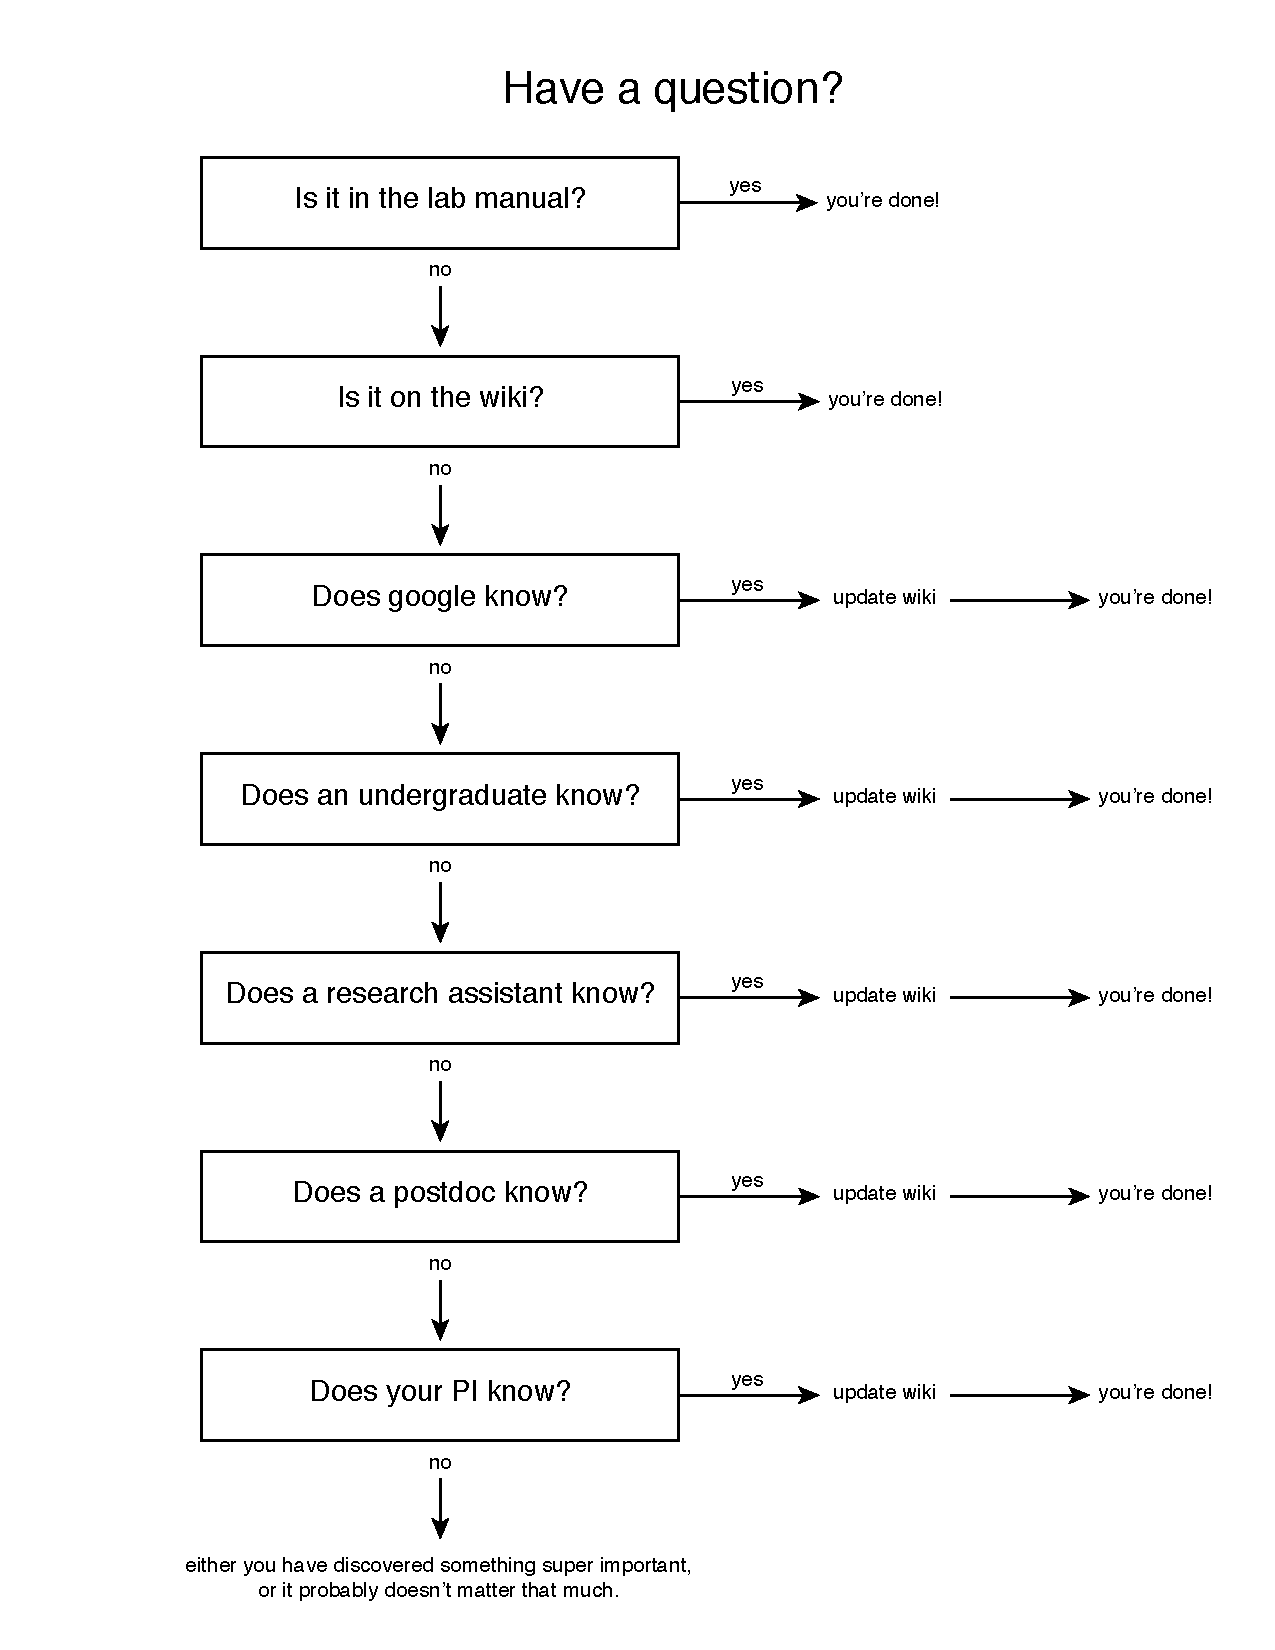
\includegraphics[width=\textwidth]{figures/lab_decision_tree.pdf}
\caption{Lab decision tree. Answers to all your questions should be in the lab wiki!}
\end{figure}

\subsection{My Door}
Metaphorically my door is always open, but sometimes my door is, physically, closed (or perhaps slightly cracked open). If this is the case:

\begin{itemize}
\item If we have a meeting scheduled, then please knock. Hopefully I am around.
\item If we don't have a meeting scheduled, a closed door generally means I am trying to do some writing and should not be interrupted. Of course, if it's an emergency, please knock anyway. Otherwise, please send me a direct message on Slack or try another time.
\end{itemize}

\subsection{Lab Meetings}
Regular lab meetings are essential for ensuring that current projects are moving forward and that future projects are being planned carefully. Remember, the lab is basically a small business that seeks to produce high-quality publications and highly-skilled trainees---i.e., you! We also use lab meetings to discuss administrative issues (e.g., IRB modifications) and practical issues (e.g., responsible conduct of research). In some case, we may also use lab meetings for workshops/tutorials that introduce or reinforce skills (e.g., using git and GitHub))

Our lab meetings are generally 1-1.5 hours. During that time, \textbf{we have one or two presenters who are responsible for setting the agenda and sharing materials well in advance of the meeting}: 1) at a minimum, one person leads a journal club on a recent empirical paper that is relevant to the lab; and 2) another person presents their work, a practice talk, a project proposal, a tutorial, or a general-interest topic that is worth a group discussion. Example general-interest topics might include a recent influential review paper, responsible conduct of research, professional development, or innovative research practices. Unless you have clinical duties or class conflicts, regular attendance and participation is expected of everyone, especially those of you working to make a sustained intellectual contribution to a project (see \Sref{sec:authorship} on \pref{sec:authorship}).

You should treat the lab meeting (and other research meetings) like a class: \textbf{be prepared, be present, and be engaged with the discussion}. This means you should read the material beforehand and avoid working on unrelated things during the meeting (which may mean putting away your laptop) because you may be called on to answer a question and/or comment on a point. If you're scheduled to present and you need to cancel or postpone, please give the group at least 72 hours notice. 

\subsection{Small-Group Data Meetings}
In addition to weekly lab meetings (mandatory), we also have small-group meetings (optional) about data, analyses, code, figures, and/or general technical issues that need to troubleshooting. In my experience, these types of discussions are much more fruitful in a group setting since others can learn and/or offer their perspective on an issue. Everyone is invited to these meetings, but nobody is \textit{required} to attend. 

\subsection{Individual Meetings}
Everyone should regularly give updates on their project(s) in lab meetings and related group meetings. In addition, everyone should also aim to meet with me individually with some regularity. These one-on-one (1:1) meetings are focused on your project(s), your goals, short-term and long-term planning, and/or challenges you are facing. Senior lab folks (i.e., postdocs, post-bacc RAs, grad students) will have these meetings on a weekly or bi-weekly basis. Please come prepared and ready to make the most of what might only be 30 minutes of time. We can cover a lot of ground in 30 minutes, and we should aim to use your Asana as the agenda.  

I generally do not set aside time regular 1:1 meetings with undergraduates because my calendar would be nothing but meetings, and I would be left with no time to get the work done that was discussed in all the other meetings! However, I am available for ad hoc meetings (see scheduling system on the wiki), and I encourage undergraduates to take the initiative and ensure that they meet with me individually at least once a semester. Come with a plan and be ready to take notes!

In general, please do not use individual meetings to discuss technical issues that would be better for a small-group data meeting. If there's a concept or technical procedure that you're struggling with (e.g., scripting first-level analyses in FSL), chances are that you are not alone and others would benefit from a quick refresher at a lab meeting. Discussing these types of things as a group helps us build expertise, improve our documentation, and develop mentors for the next generation of trainees who will have the same questions (see \Sref{sec:training} on \pref{sec:training}). 

\subsection{Slab: The Lab Wiki}
\label{sec:wiki}
%(see \Sref{sec:wiki} on (\pref{sec:wiki})

Anyone reading this document is probably familiar with Wikipedia, which is an encyclopedia whose content is collaboratively edited and improved by the world. But what is a ``wiki"? Here's a definition\footnote{\url{https://en.wikipedia.org/wiki/Wiki}}:

\begin{displayquote}
A wiki is a hypertext publication collaboratively edited and managed by its own audience directly using a web browser. A typical wiki contains multiple pages for the subjects or scope of the project and could be either open to the public or limited to use within an organization for maintaining its internal knowledge base.
\end{displayquote}

In our lab, we use a web-based program called Slab to host our wiki. The lab wiki is our shared collection of knowledge about how to get things done in the lab. The lab manual you are reading now is ``top down'', in that I am writing the whole thing myself. By contrast, the wiki is a shared resource to which everyone can---and should---contribute. A good rule of thumb is that if you need to figure out how to do something, someone else in the lab will someday need to do the same thing. Whenever possible please document what you figure out on the wiki, including updating old sections which may no longer be relevant. Please encourage each other (and those working with you) to do the same!

Minimally, I expect you to improve existing documentation on the wiki as needed and also maintain pages that are specific to your projects. Your project page(s) will detail all of the relevant aspects of your project that would allow someone else (e.g., you in 6 months, a new trainee in 2 years, me in 5 years, etc.) to reproduce what you are doing. You can build off examples from others', but it's very important to keep it up to date and add notes and insights and they materialize. Thus, your Slab page for your project will also serve as your shared lab notebook that will certainly help others when one of your insights comes up in one of their searches. Remember, share your knowledge and use the wiki to facilitate that process.


\subsection{Asana and Slack}
Asana and Slack are the main tools for lab communication and are preferred to email in almost every situation. Please help me by keeping these up to date! A few thoughts and tips (find more on the Lab Wiki):

\begin{itemize}
\item Asana is just a shared to-do list, which makes it easy to use. My advice is to keep it simple: add a task, a description, due date, and tag whoever needs to know about its status. Then work toward completing that task, adding comments (updates or questions) as needed to get the job done.
\item Be realistic and flexible with due dates in task in Asana. Of course, you should try to get things done in a timely manner---while recognizing that some tasks necessarily have to be completed before other tasks---but sometimes life happens and you have to adjust.
\item In Slack, try to avoid direct messages for project-related discussions or questions. These questions can generally be asked in an open channel that others can see. Also, when using Slack, please use threads to help keep conversations organized and avoid spamming others.
\item Use the default settings for notifications in Slack and Asana (though cut off sounds, please!). They are defaults for a reason. But, if the extra emails clutter your Inbox, take a few minutes to set up a filter.
\item Use Asana and Slack together. You can integrate them with a few simple clicks. I will often create and assign tasks directly from Slack\footnote{If you wind up with multiple Asana accounts tied to different emails, you should integrate them to save extra work and avoid confusion.}.
\item Did someone miss a message on Slack or a task on Asana? Don't hesitate to follow up, bring it to me, raise at lab meeting, and/or mention it in person.
\end{itemize}

\begin{shaded}
\noindent I have a love-hate relationship with Slack. While I prefer it over email for lab communication and announcements, I've noticed that it can be easy for folks to miss messages, depending on their settings and individual habits. So, don't be shy about voicing your opinion about what would optimize the signal to noise ratio on each of our Slack channels. In general, using Slack---or any tool for communication---should not be a real barrier for your progress or growth.
\end{shaded}

\subsection{Email}
When contacting me, please use Asana/Slack whenever possible. I will try to reply to emails when I can but please don't use it for anything urgent if you can avoid it. If you need to reach me urgently you can call/text my cell phone, or call the lab (where someone can get in touch with me). 

I would like to use Asana/Slack as much as possible for lab communication, but sometimes I will need to email you. I expect you will read all email sent to you and respond (if a response is needed) within one business day. If you're not going to be checking email for more than a few days (for whatever reason), please consider using a vacation message so that others know you're not on email (this suggestion also applies to holidays). The same guidelines apply to me: if I don't respond to one of your messages within one business day, please feel free to follow up; and if I'm not checking email at all, I will put up a vacation message. 


\subsection{Calendars}
Accurate calendars are extremely important in managing lab space and resources. We have a Lab Attendance calendar (for noting when you're away) and there are other calendars for other purposes (e.g., booking the scanner). It is crucial that everyone use the calendars regularly and ensure they are accurate. Use the lab calendars and follow the instructions described on the wiki.

Of course, you should also maintain your meetings and other commitments in your own calendar. When I set up a meeting with you, you will often get a calendar invite email. Once you click the ``yes'' or ``accept" button, that event is in your calendar and there will be little to no confusion about the meeting time. 




%%%%%%%%%%%%%%%%%%%%%
\section{Communication Outside the Lab}

Communicating to people outside the lab is extremely important: your actions reflect not only on yourself, but on the lab, the lab director, the department, and the university. This is true both for participants (who volunteer for our studies) and scientific colleagues (whose opinions have a direct impact on our success and opportunity---they are the ones reviewing our grants and papers!). It is important that every time one of us represents the lab to a high level of quality. The less experience you have, the more preparation is required. Don't skimp!

\subsection{Phone}

\begin{itemize}
\item If the phone rings in the lab, answer it: identify the lab and your name. Most calls will be from potential (or current) research participants, so it's important they view us as professional and competent. ``Smith Lab. This is [your name here]. How may I help you?'' is a great start. 
\item Check voicemail messages daily to make sure nothing important slips through.
\item If someone calls the lab and leaves a message, call them back within one business day to confirm that we received the call. If they would like to participate in a study but we can't schedule them, thank them for their interest and ask if we can contact them in the future should one come up (if you actually will). If you are not going to contact them (or they do not qualify), tell them that we are done recruiting for that study and do not have anything else available, but thank them for their interest. Refer to \Sref{sec:participants} (\pref{sec:participants}) and the lab wiki for detailed instructions on scheduling participants and general phone etiquette.

\end{itemize}


\subsection{Manuscripts}
Scientific papers are one of the principal product of the lab. Both the quantity and quality of our papers have a direct impact on the success of the lab and serve as critical way for you to showcase your talents to those outside the lab. Together, we should strive to publish and prosper. 

\subsubsection{General}
\label{sec:ms_general}
%\Sref{sec:ms_general} (\pref{sec:ms_general}

We have an obligation to communicate our findings clearly and unambiguously. However, clear and unambiguous communication can be challenging, especially when writing a manuscript. Before you sit down to write a manuscript, I expect you to be familiar with what George Gopen calls \href{https://cseweb.ucsd.edu/~swanson/papers/science-of-writing.pdf}{``Reader Expectations"}. These are just general principles, but I encourage you to read some of the books we have in lab if you want to master this important skill. 

With these principles in mind, here are some additional guidelines for drafting a manuscript in the Smith Lab:

\begin{itemize}[noitemsep]
\item Always start with paragraph-level outlines of each section that include the key citations and points you intend to make.
\item Obsess over flow, context, and structure.
\item Remember that the reader does not know what you know.
\item Always show a manuscript (or revision) to all authors before submitting it, giving them the opportunity to comment.
\item Go over page proofs carefully, including the references. There is almost always a mistake (ours, or introduced by the publisher).
\item Always give the senior author the opportunity to look at page proofs.
\end{itemize}


\subsubsection{Formatting}

When you are out in the big world on your own, you are free to format your manuscripts however you like. While you're in the Smith Lab, when sending me a draft of a manuscript, please do the following:

\begin{itemize}[noitemsep]
\item Include a title, or multiple options for a title, if you are unsure. 
\item Include page numbers.
\item Include the full author list starting from the first draft, which helps clarify any authorship issues or concerns early on.
\item Include placeholders for all sections (e.g., introduction, methods, results, discussion.) even if they are empty, so that we can fill them in as we go. Having placeholders also helps clarify the organization from the beginning.
\item Use styles, especially for headings. This will help organization of the manuscript and make it easy to change font and formatting if need be. (To make a heading, don't simply select the text and make it bold; select the text and then a heading style, such as ``Heading 1''.)
\item While we are sending drafts back and forth, keep the text single-spaced. If the journal requires double spacing, we can add this at the end.
\item Embed figures and tables in the body of the manuscript rather than putting at the end, or in separate files. Again, we can change this to match journal guidelines before submitting if need be.
\end{itemize}

Some of these are good practice; others are simply my own preferences. However, if you humor me in these, it will decrease my distraction when reading your writing, and ultimately enable me to be more useful.

Your papers should be free of spelling and grammatical errors. There is no shame in asking for help with this; your fellow labmates, classmates, or the writing center (\url{http://www.temple.edu/writingctr/}) are available to help. The best proofreaders will explain to you \textit{why} things need to be changed so that you learn how to be a better writer, rather than simply correcting your writing. 


\begin{shaded}
\noindent We're moving past the days of having to add version numbers to MS Word files since we use the lab OneDrive. But if you're not using the lab OneDrive and you're sending files back and forth, please include your name and a version number. If you send me a file called ``Research\_Statement.docx'', it is likely to get lost---try ``Baldrick\_research\_statement\_v01.docx'' (assuming your name is Baldrick and this is the first version you are sending me). In either case, be thoughtful about how you name files: file names should be both human and machine readable (see more \href{http://www2.stat.duke.edu/~rcs46/lectures_2015/01-markdown-git/slides/naming-slides/naming-slides.pdf}{here)}.
\end{shaded}

\subsubsection{Figures}
If we are still trying to work out what a good figure looks like, I'm happy to talk this through with you and look at rough drafts. However, if we have a good idea of what we want in the figure, please send me something as finished and polished as you can make it---this makes it easy for me to give the most helpful feedback. If you give me something that isn't your best work, I will probably just tell you things you already know.

Most figures should be vector art (saved as PDF or EPS files). Vector-based files don't suffer the artifacts and poor quality that raster-based images show when magnified. Use a graphing program (such as R, Matlab, or JASP) to export to an EPS file, and then modify that file in Adobe Illustrator or other vector-based image-editing program (e.g., Inkscape).

\begin{shaded}
\noindent Don't use Microsoft Excel or Microsoft Powerpoint for your figures! They are never the best option. If you must organize your data in Excel, that's fine, but then do plotting in a better plotting program (e.g., R, Matlab, or Python).
\end{shaded}


\subsubsection{Corresponding Authorship}
On average, I am around the longest and have the best chance of having access to data, etc. To keep the rules the same for everyone I am always corresponding author for research conducted in the lab.



\subsection{Conference Presentations}
I encourage everyone in lab to seek out conferences and meetings that would be a good venue for your work (a list of possibilities can be found on the wiki). Anyone submitting an abstract for a conference, symposium, etc. should clear this with me first, and circulate to all authors at least one week before the submission deadline.

\subsubsection{Talks}
Anyone giving a talk to a non-lab audience is required to give a practice talk to the lab at least one week before the real talk. If this is your first public talk on a lab project, plan on at least two practice talks (starting at least 2 weeks before the real talk). Practice talks should be mostly finished (final slides, practiced, and the right length) so that our comments will be as helpful as possible. Schedule one or more meetings with me ahead of time to plan or go over your slides, especially if you haven't given many talks before. You should \textit{never} have to stay up late finishing a talk.

\subsubsection{Posters}
Anyone presenting a poster should circulate an initial version to all authors at least one week before the printing deadline---which can be up to a week before you plan to leave for the conference (plan accordingly). If it's your first poster, plan to present it to the lab before you print. 

Make sure to double check the poster size and orientation for the conference, and the size of the paper or canvas it will be printed on.

For many conferences, you may want to bring a sign-up sheet where people can request an emailed PDF. However, these sign-up sheets can be difficult to read, so you could also print a QR code on your poster that links to your poster and/or include an OSF link to your poster.

\begin{shaded}
\noindent Plan ahead and be prepared when it comes to conference presentations. If you're unprepared or if you're unprofessional during a conference, then I will be much less likely to send you to conferences in the future. Likewise, if you submit an abstract with preliminary results and don't make sufficient progress toward finalizing those results before the conference, we may withdraw your submission since the feedback at the conference may not as helpful as we'd like.
\end{shaded}

% \Sref{sec:participants} (\pref{sec:participants}) 

\section{Communication with Everyone}
Everything we do should be sharable with other researchers and the public. I want everyone to assume that all of their notes, instructions, de-identified data, and results will be publicly-accessible on the OSF and/or GitHub in the near future (see \Sref{sec:openscience} on \pref{sec:openscience}). 

\subsection{Open Science Framework}
We try use the Open Science Framework (OSF) for organizing (and sharing) materials and documentation related to our projects. For example, OSF may be used for submitting a pre-registration, sharing materials, and/or posting a preprint. At the end of the day, it is easy enough to simply link your OSF project to the current \href{https://osf.io/myxet/}{Smith Lab} page to help keep everything together and easy to find when necessary. The reason we do this is simple: If someone contacts me for additional information about one of our projects, my hope is that I can easily find the correct OSF page and send them a link with everything. And in an ideal world, this OSF link will already be in your paper and nobody will ever have to request our materials. 

\subsection{GitHub}
We use GitHub to version control and share code that is tied to our analyses and/or stimulus presentation. You can link your GitHub repository to OSF. 


%%%%%%%%%%%%%%%%%%%%%
\chapter{Science}

\section{Scientific Integrity}

You have a responsibility to me, the institutions that support our work, and the broader scientific community to uphold the highest standards of scientific accuracy and integrity. By being in the lab you agree to adhere to professional ethical standards. There is never an excuse for fabricating or misrepresenting data. If you have any questions, or in the unlikely event that you have concerns about a research practice you have seen in the lab, please talk to me immediately.

It is also important that you prioritize the accuracy of your work while in the lab. Unintentional errors due to inattentiveness or rushing can be extremely damaging and produce results that turn out to be incorrect. Mistakes will happen, so please double-check your work frequently. In many cases, multiple people will double-check a dataset or workflow to ensure no mistakes have crept in along the way.

When collecting data, please use simple checklists to ensure that everything gets done and has someone who is responsible for each specific aspect of your protocol. You should also \textit{analyze data as soon as you collect it} to ensure that it was collected properly!


\section{Open, Accurate, and Reproducible Science}
\label{sec:openscience}

\subsection{Open Science \& Reproducibility}

We are working towards putting all stimuli, data, and analyses online and linked to each research publication. The idea is not to simply tick a box of ``open science'', but to make these resources readable and useable for reviewers and other researchers. In service of this:

\begin{itemize}
\item All files should be named and organized according to the \href{https://bids.neuroimaging.io/}{Brain Imaging Data Structure} (BIDS) standard.
\item GitHub pages should have a README.md\footnote{The content of these files can automatically be linked to Slab, which makes sharing knowledge with others in lab much easier!} file that describes what is in the repository and how to use the repository. In all cases, make sure your documentation provides enough information for an outside reviewer/collaborator to reproduce what you did without consulting you.
\item Code should be tested, bug-free, and (helpfully) commented, with reproducible results. For tips on documenting code, check out this \href{https://journals.plos.org/ploscompbiol/article?id=10.1371/journal.pcbi.1006561}{``10 Simple Rules" paper by Benjamin Lee}.
\item Links should be permanent, ideally a DOI---which we can obtain through the \href{http://help.osf.io/m/sharing/l/524208-create-dois-and-arks}{OSF}, \href{https://figshare.com/}{FigShare}, or \href{https://zenodo.org/}{Zenodo}.
\end{itemize}

In pursuit of this high level of organization and documentation, lab members will frequently be asked to review and error-check lab materials (including text lists of stimuli, code input/output, etc.) and reproduce results. Lab members creating stimuli or conducting research projects should organize them from the outset in a way that is conducive to eventual sharing (GitHub, OSF, Jupyter notebooks, etc.).


\subsection{Accurate Science}

A key part of accuracy is anticipating and avoiding problems, and creating structures in the lab that facilitate a high level of reliability. We will make mistakes, but we must learn from them and avoid repeating them.

Inspired by Jeff Rouder's 2019 paper titled \href{https://doi.org/10.1177/2515245918801915}{Minimizing Mistakes in Psychological Science}, we have a page on the lab wiki for documenting previous problems and potential new ones. Whenever new information is added to this page, we it will be discussed at lab meeting to make sure none slip through the cracks. Examples of problem events include:

\begin{itemize}
\item Any of the lab computers malfunctioning
\item Any data analysis/transfer procedure not working correctly (e.g., downloading imaging data from XNAT)
\item Not being able to find the installation disc for a software program
\item Nearly running out of money to pay participants (this counts as a ``near miss'' which we also need to discuss)
\end{itemize}

As a lab member it is your responsibility to be aware of times when things don't go as planned and bring these to the attention of the rest of the group. Even better, let's all work together to find ways of preventing such occurrences in the future.




\section{Participants}
\label{sec:participants}

Our research is made possible by the goodwill and generosity of our research participants. We not only need people to participate in our studies, but to try hard to do their best, and potentially return for a future study. Caring for our participants is one of the most important parts of the lab and something in which every member plays a role.

The most important thing is that participants must always be confident that we are professional and treating them with respect. All of the specific advice supports these goals. In general, it is helpful to model our interactions off of other professional situations, such as a doctor's office.

For all participants:

\begin{itemize}
\item Dress professionally: No jeans, t-shirts, sweatshirts, sneakers, or sandals. When in doubt, ask! This is true for both young and older adults---dressing professionally will help undergraduate participants to take the experiment seriously.
\item Answer the phone, and return all phone calls (and emails) promptly. Tell participants who you are, and where you are calling from: ``Hello, this is [name] calling from the Smith Lab at Temple University. I am returning your call from yesterday regarding a research study.''
\item Task instructions must be extremely clear. Ensure that the participant understands that their choices really impact the amount of money that they take home (i.e., their decisions must be incentive compatible). 
\item Be prepared to answer questions. If you don't know the answer, it is completely fine to ask the participant if someone else can call them back. You are then responsible for making sure this happens quickly.
\item Arrive at least 30 minutes prior to testing time to make sure equipment and paperwork are all set, and to be around in the event the participant shows up early. Everything should be set up before the participant arrives. For people coming from off campus, you should be at the designated meeting spot 15 minutes before the agreed upon time.
\end{itemize}
	
For non-students, and especially older adults, always use a title (Dr./Ms./Mr.) and a participant's last name when addressing them. If you aren't sure how to pronounce their name, ask them.

We can also help participants feel more at ease by being thoughtful about the language we use. For example, participating in a ``research study'' is more friendly than being a ``subject'' in an ``experiment'' (e.g., see Table \ref{table:terms}).

% table for research terms
\begin{table}
\centering
\caption{Terms associated with research studies}
\begin{tabular}{ll}
\toprule
Instead of saying: & Say this:\\
\midrule
experiment& study, research study\\
subject& volunteer, participant\\
test & task or screening or game \\
\bottomrule
\end{tabular}
\label{table:terms}
\end{table}

Refer to the lab wiki for specific information on recruiting, scheduling, and testing participants.


\section{Subject Payment}
\label{sec:subject_payment}

We pay our subjects with various forms of payment cards and cash. One of the lab members checks out the money, and then people testing participants will take out what they need to pay the subjects. Each subject signs a payment sheet and receipt booklet to document that they got paid. Naturally, it is very important that we keep track of this money.



\section{Testing Locations}
\label{sec:testing_locations}

\begin{itemize}
\item Some of our shared testing locations are shared with other researchers, so it is very important that we are good citizens when it comes to using these spaces. Being a good citizen includes scheduling the time as required, not using more than our allotted time, and leaving the room as clean as we found it (or preferably cleaner).
\item No Smith Lab equipment should be left in shared testing rooms---this includes laptop, stimulation device, etc. (It all lives in the lab.)
\item No one should test a subject without signing out the testing room.
\end{itemize}



\section{Lab Notebook}
\label{sec:lab_notebook}

Anyone conducting an independent research project should have a lab notebook for keeping track of discussions, experiments, and taking notes. In practice, your Lab Notebook will probably consist of handwritten notes on a piece of paper, your comments in Asana, and your project page in Slab. At the end of the day, I don't care where you initially store your notes, but it is very important that all of your project-related notes and insights make it to your project page on the wiki. Again, this helps you effortlessly share your knowledge and insights with your lab mates (and yourself 6 months from now). 

\section{Computers and Data}

\subsection{General Guidelines}

\begin{itemize}
\item Testing laptops should never leave the lab except for testing. Always sign out the computer and any other equipment on the lab wiki.
\item Do not install extraneous software or store personal files on the computers.
\end{itemize}

\subsection{Backing Up Your Files and Data}

Always assume that as soon as you turn your back the computer on which you have been working will explode.Thinking such dire thoughts will make it easier to follow these guidelines:

\begin{itemize}
\item If you save files to the shared lab drive (the S drive), backup will automatically happen. 
\item Data from participants is irreplaceable and should be removed from testing computers immediately following testing and onto the lab OneDrive.
\item \textbf{Be sure to constantly push changes to scripts up to GitHub}. Your scripts and code are almost as valuable as participant data. There is no excuse for losing scripts or code, so please use GitHub for everything, though you must ensure your commits are restricted to code and de-identified data.
\item When working on manuscripts, be sure to use the lab OneDrive so that your files are backed up and accessible anywhere.
\end{itemize}


\section{Authorship}
\label{sec:authorship}
%\Sref{sec:authorship} (\pref{sec:authorship}

Many professional associations and journals have published authorship guidelines, which are worth looking at (for example: \href{http://www.icmje.org/recommendations/browse/roles-and-responsibilities/defining-the-role-of-authors-and-contributors.html}{ICMJE}). Many of these guidelines call for a sustained intellectual contribution; and in my view, there are two key requirements to being an author:

\begin{enumerate}
\item Contribute to the intellectual scientific content of the manuscript in a meaningful way.
\item Contribute to the writing of the manuscript in a meaningful way.
\end{enumerate}

Note that ``collect data'', ``analyze data'', or ``fund the study'' aren't on the list. Those are very important parts of a paper, but do not (on their own) warrant authorship. Being an author means understanding the content and being willing to take public responsibility for the work: a large part of this concerns the theoretical motivation and implications of the research. In practice, theoretical contributions are most often made through helping with the study design, data interpretation, and discussion about a topic.

Also note that being an author on a poster (or abstract) at a scientific meeting does not automatically make you an author on the paper. The thresholds for authorship on a poster vs. a paper are very different, and I will often be much more inclusive when it comes to posters coming out of the lab\footnote{In general, anyone who has helped with data collection/analysis over the course of at least one semester may be included as authors on posters.}.

This doesn't mean that as an undergraduate student or research assistant you can't be an author on a paper. Of course, if the study goes well and you are involved, you might be. However, you will need to know enough (or learn enough) about the subject to understand what we've done, and to significantly contribute to the writing. I won't add you to a paper just because I like you and want to help you out; I {\itshape will} consider giving you the opportunity to be involved to a degree that you have earned authorship, if you are willing to take on the challenge.

Typically one person will take on the main responsibility for writing the paper, and this person will be the first author. However, as noted above, I expect all authors to contribute to the writing of the manuscript. This contribution could take the form of helping structuring arguments, identifying key citations, and developing paragraph-level outlines. Once we have clear, paragraph-level outlines, it is easier to split some of the writing responsibility (e.g., a minor author might be more able to write a specific paragraph in the Discussion, if it is more within their expertise).

As papers work their way through the lengthy publication process (which can be years), it is sometimes possible that authorship may change in a way that reflects the overall intellectual contribution up to publication. For instance, if you're the first author on the initial submission and then you subsequently bail and someone else does all of the work to see it published, we will need reconsider authorship order.

With respect to authorship order---and authorship more generally---it can be instructive to think of a histogram plotting the number of hours invested into making a sustained intellectual contribution. Naturally, the first author will have the largest investment. However, it is not unreasonable to see that the 2nd author is putting in at least half as much time as the 1st author. In cases where there's no clear difference between 1st and 2nd author, we can consider assigning co-first authorship (this should be a relatively rare phenomenon). Most papers coming out of the lab will have at least 3 authors and all authors will play an essential role in developing the final product.

I assume that, unless we have talked about it, I will be an author on papers coming out of the lab. This does not mean that you should add me on to papers as a courtesy; it means that I expect you to include me in the process of discussion and writing in a way that merits authorship. In other words, the same approach I take with you.

It is worth pointing out that there are many views regarding authorship, and within any view there are always borderline cases. When collaborating with other people, I tend to defer to their own lab culture. However, it's important that within our own lab, we are clear on the expectations for authorship and transparent about authorship discussions and decisions. If you ever have any questions, please come speak to me.


%%%%%%%%%%%%%%%%%%%%%
\chapter{Other Important Information}
\section{Recommendation Letters}
It is part of my job (and, thankfully, quite often a pleasure) to write strong letters of recommendation for people in the lab. Please give me as much notice as possible (e.g., at least one month), and make sure I know the deadline, official name of the organization, what you are applying for, and so on. Please also send along a current CV and any specific talking points or examples you want me to highlight. Like everything else, communication is key, and when in doubt, ask!

\section{Staying on Top of the Literature}
\label{sec:literature}

Anyone who is trying to make a sustained intellectual contribution to a project (see \Sref{sec:authorship} on \pref{sec:authorship}) should be spending a good chunk of time each week reading and thinking about the literature tied to that project. Dozens of relevant papers come out each month, so it becomes challenging to read everything. At Temple and in the Smith Lab, we have regular discussions of journal articles. These discussions happen through our weekly lab meeting and various journal clubs that you should hear about via the weekly events email sent by the department. Please attend these meetings when it is applicable to your work and contribute to the discussions. When you're reading papers (or even just skimming abstracts), think about the following questions:

\begin{itemize}
\item Which papers are ``good" and ``bad" (and why)? This question will be hard to answer at first. That's ok. You will get better with practice. In fact, you can now target this critical thinking skill by reading journals that publish the reviewer reports alongside the paper (e.g., \textit{eLife, European Journal of Neuroscience, Nature Communications}).
\item How exactly do the papers relate to our lab in general and to your project(s) specifically?
\item How do different papers agree/disagree with each other?
\item How do the papers contribute to big-picture questions in the field? 
\item What questions do the papers create?  
\end{itemize}

There are many different strategies for staying on top of the literature. For years, I've received Table of Content (TOC) emails from various journals each time there's a new issue of the journal. I also get a lot of information from Twitter, \href{http://pubcrawler.gen.tcd.ie/}{PubCrawler} alerts, and from Google Scholar alerts for specific authors---and I share much of what I see directly to one of the `papers-*` channels on Slack (you should share what you see, too!).

But, all of these articles can really be overwhelming. So, how can you manage all of this information? Here are my recommendations:

\begin{itemize}
\item Budget time for reading papers and synthesizing information, especially when you are in the early days of exploring a new topic or question. 
\item Set up alerts for \textit{some} journal TOC emails and use PubCrawler and Google Scholar for term- or topic-specific alerts. Also follow folks on Twitter (or related social media). There are lots of smart people on social media who act as filters and disseminate articles (and other information) that you may find useful.
\item Use reference managing software, such Zotero (free). These programs will help you collect references, add notes, and organize them however you like. 
\item Set aside time to review what you've added to Zotero and think about how those papers fit together.
\item Force yourself to write a couple of cohesive paragraphs each month that connects the dots on some of your favorite recent papers. You should be able to use this paragraph in a future class or paper; but even if you can't immediately, you will have at least spent some time practicing your writing and getting your head around multiple papers.
\item Share what you're reading and thinking about during lab meetings. Whenever you present an article or your own data, use it as an opportunity to connect with the literature and share information with others. 
\end{itemize}

\begin{shaded}
\noindent The bottom line is simple: You need to read a lot and be able to synthesize different pieces of information. In science, everything is connected; but in order to see those connections---or design the experiments that will create the connections---you must know the literature like the back of your hand.
\end{shaded}


\section{Learning to Code}
\label{sec:coding}

Computer programming (i.e., coding) is an essential skill that all students within psychology and neuroscience should develop\footnote{\url{http://www.russpoldrack.org/2016/05/advice-for-learning-to-code-from-scratch.html}}. Being comfortable with computer programming---especially Python and Matlab---will enable you to develop your own task scripts and wrangle data. 

Yet, learning computer programming can be a challenging task. In most situations, you will not learn how to code from psychology/neuroscience classes at Temple. Instead, you will learn from online training materials, software manuals/tutorials, other trainees, and your own experiences. Having a specific problem or goal in mind (e.g., program a new task or analyze a new dataset) helps considerably. While you're learning to code, keep the following points in mind:

\begin{itemize}

\item Be patient and persistent. No one ``gets it'' immediately, and you may have to work through several errors before arriving at a solution. 
\item Be careful and obsessive. Most coding mishaps occur because of a tiny typo. If you're careful and thorough, you will catch these mistakes and save yourself time and frustration. 
\item Understand input and output for all scripts you use.
\item Have a basic sense of how each line of code relates to other lines of code in your script. Everything is connected. 
\item Paths errors are common. Avoid them by shoring up your understanding directory structures. Every input and output file lives in a specific location that you control. 
\item Avoid staring at the same error for more than 30 minutes. If you haven't solved it in 30 minutes, switch to some other work or take a walk outside.
\item \textbf{Don't be shy about asking for help.} Other students/trainees and internet forums (e.g., NeuroStars) are great places to find help. You can also post a quick message to the `troubleshooting' channel on Slack.

\end{itemize}


\begin{shaded}
\noindent Although learning to code can be a daunting and frustrating task, it is well worth the investment. Coding is a skill that will generalize well beyond the laboratory, particularly industry positions involving data science. 
\end{shaded}


\section{Effective Menteeship}

If you've been in the lab for a semester (or even just a few weeks in some cases), you should have learned enough to teach and mentor others who are more junior. But that doesn't mean you don't need further mentorship and guidance. Indeed, virtually everyone---including your PI---functions as a both a mentor and mentee. Although much has been written and said about what makes a good mentor \href{https://doi.org/10.1016/j.amjmed.2010.12.007}{(e.g., Cho et al., 2011, A J Med)}, relatively less has been said about what makes a good mentee. 

So, how can you be an effective mentee in the lab? I didn't really consider this question deeply or explicitly until I got involved in a Mentor/Mentee matching program (2022-2023) sponsored by the Organization for Human Brain Mapping\footnote{OHBM Program: \url{https://doi.org/10.1111/ejn.14320}}. At the beginning of the program, they shared some resources for how to be a good mentor and how to be a good mentee. For example, \href{https://doi.org/10.1136/bmj.i4147}{Chopra and colleagues (2016, BMJ)} write about the ``golden rules of effective menteeship," and I encourage you to read their article. That article outlines why and how mentees can do the following things to get the most out of their mentor(s):

\begin{itemize}
\item Be respectful of your mentor’s time and manage it wisely
\item Communicate efficiently and effectively with your mentor
\item Be engaged, energizing, and collaborative
\end{itemize}

I think this is all sound advice and makes good sense (perhaps at the risk of sounding obvious). One theme is ``managing up," which basically means the mentee takes ownership over the relationship, a concept that is echoed in similar work \href{https://doi.org/10.1097/ACM.0b013e3181906e8f}{(Zerzan et al., 2009, Academic Medicine)}. Of course, some folks ``manage up" and do these things automatically in all professional situations, but others may find it to be novel and helpful advice. Either way, I think effective menteeship---like effective mentorship---is a learned skill that requires practice, patience, and trial and error.



\end{document}